% Chapter 2

\chapter{Diseño del hardware y software}
\label{Chap:DisHard} % For referencing the chapter elsewhere, use \ref{Chapter2} 

%----------------------------------------------------------------------------------------

\section{Introducción}

En este capítulo se presenta información referente al funcionamiento general del sistema. Se divide en dos secciones: el hardware y el software, donde en cada uno se muestran diagramas o imágenes de funcionamiento, junto a una breve explicación.\\

En el diagrama de la figura~\ref{fig:diagcomp} se muestran los componentes de cada una de las estaciones.

\begin{figure}[H]
\centering
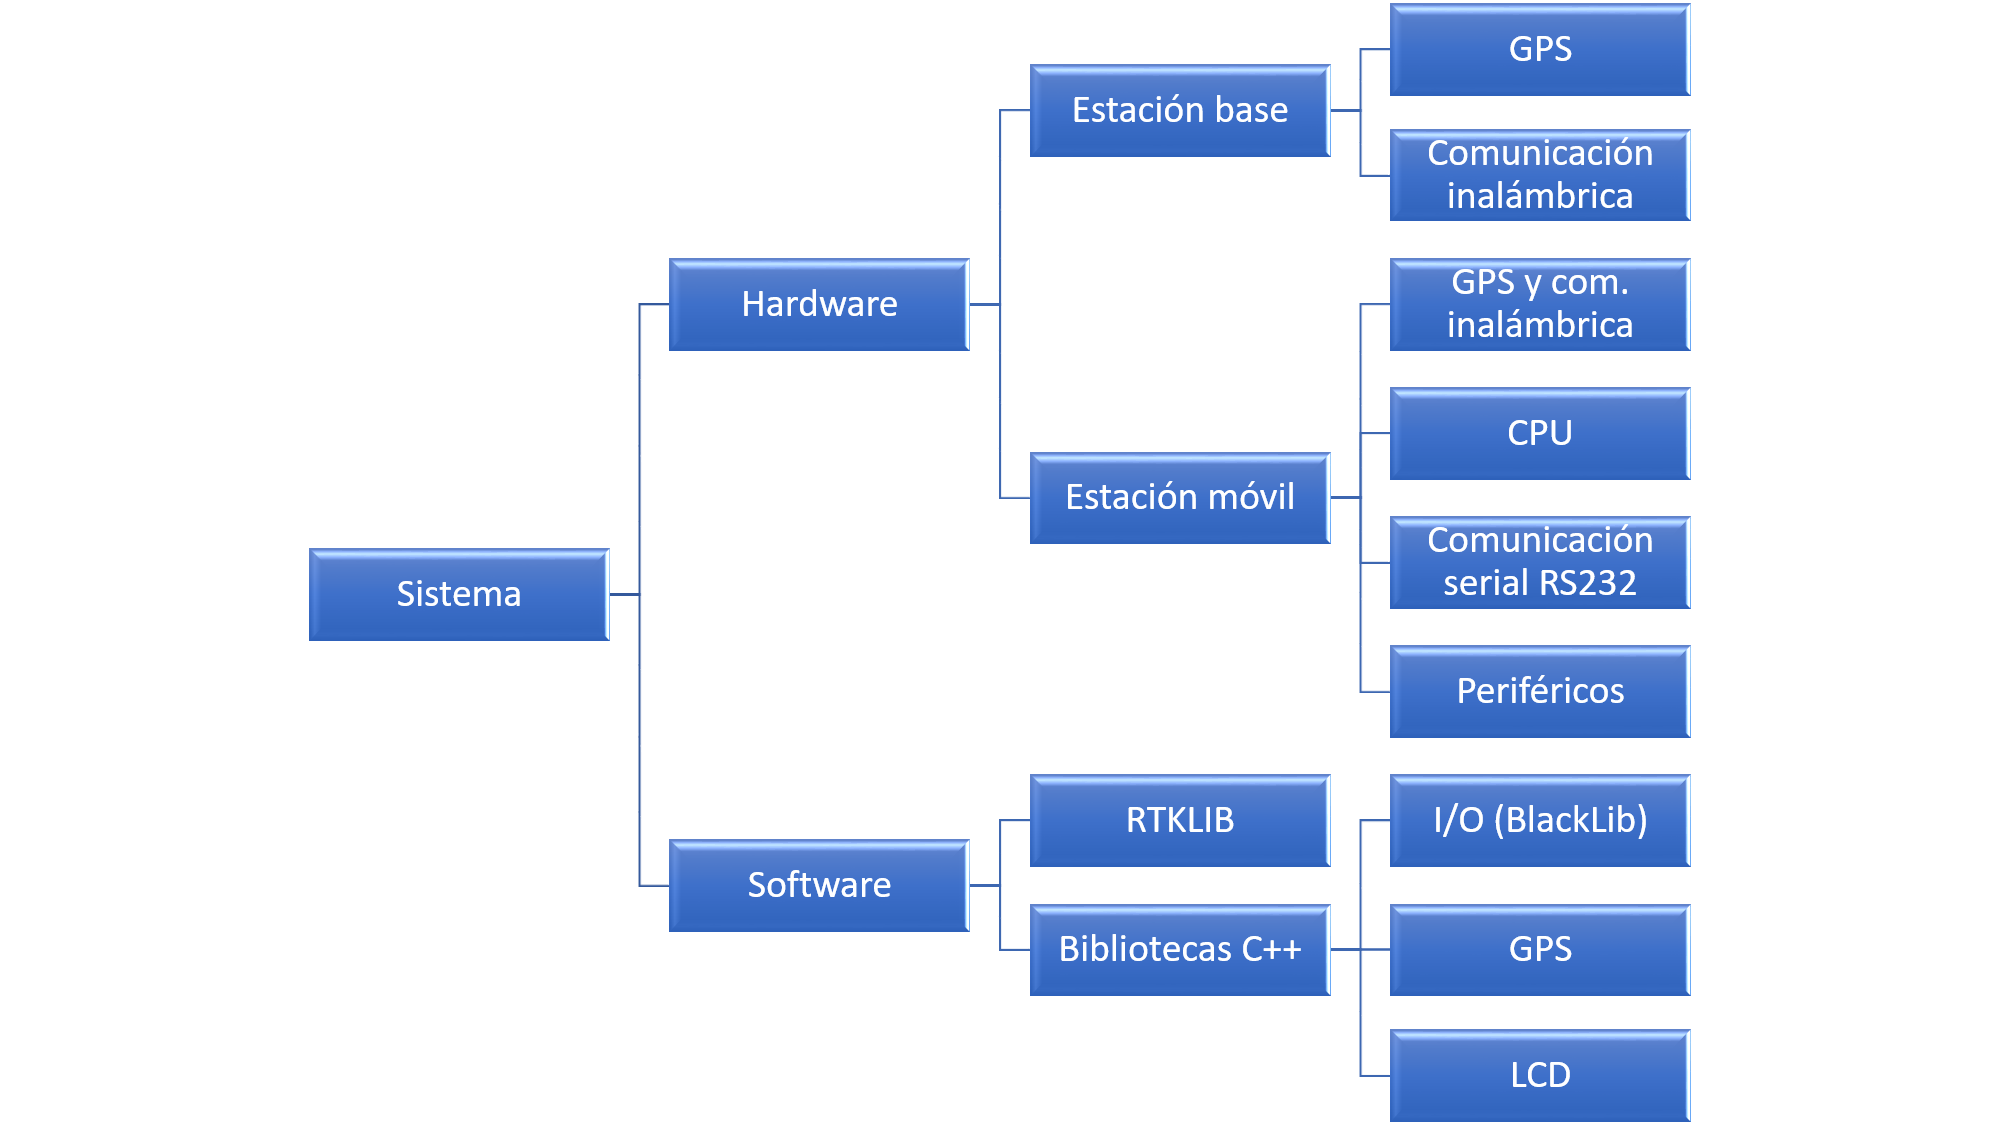
\includegraphics[width=0.95\textwidth]{Figures/DiagramaFinal}
\caption[Diagrama de componentes.]{Diagrama de componentes.}
\label{fig:diagcomp}
\end{figure}

\section{Hardware}

\subsection{Prototipo}

\begin{figure}[H]
\centering
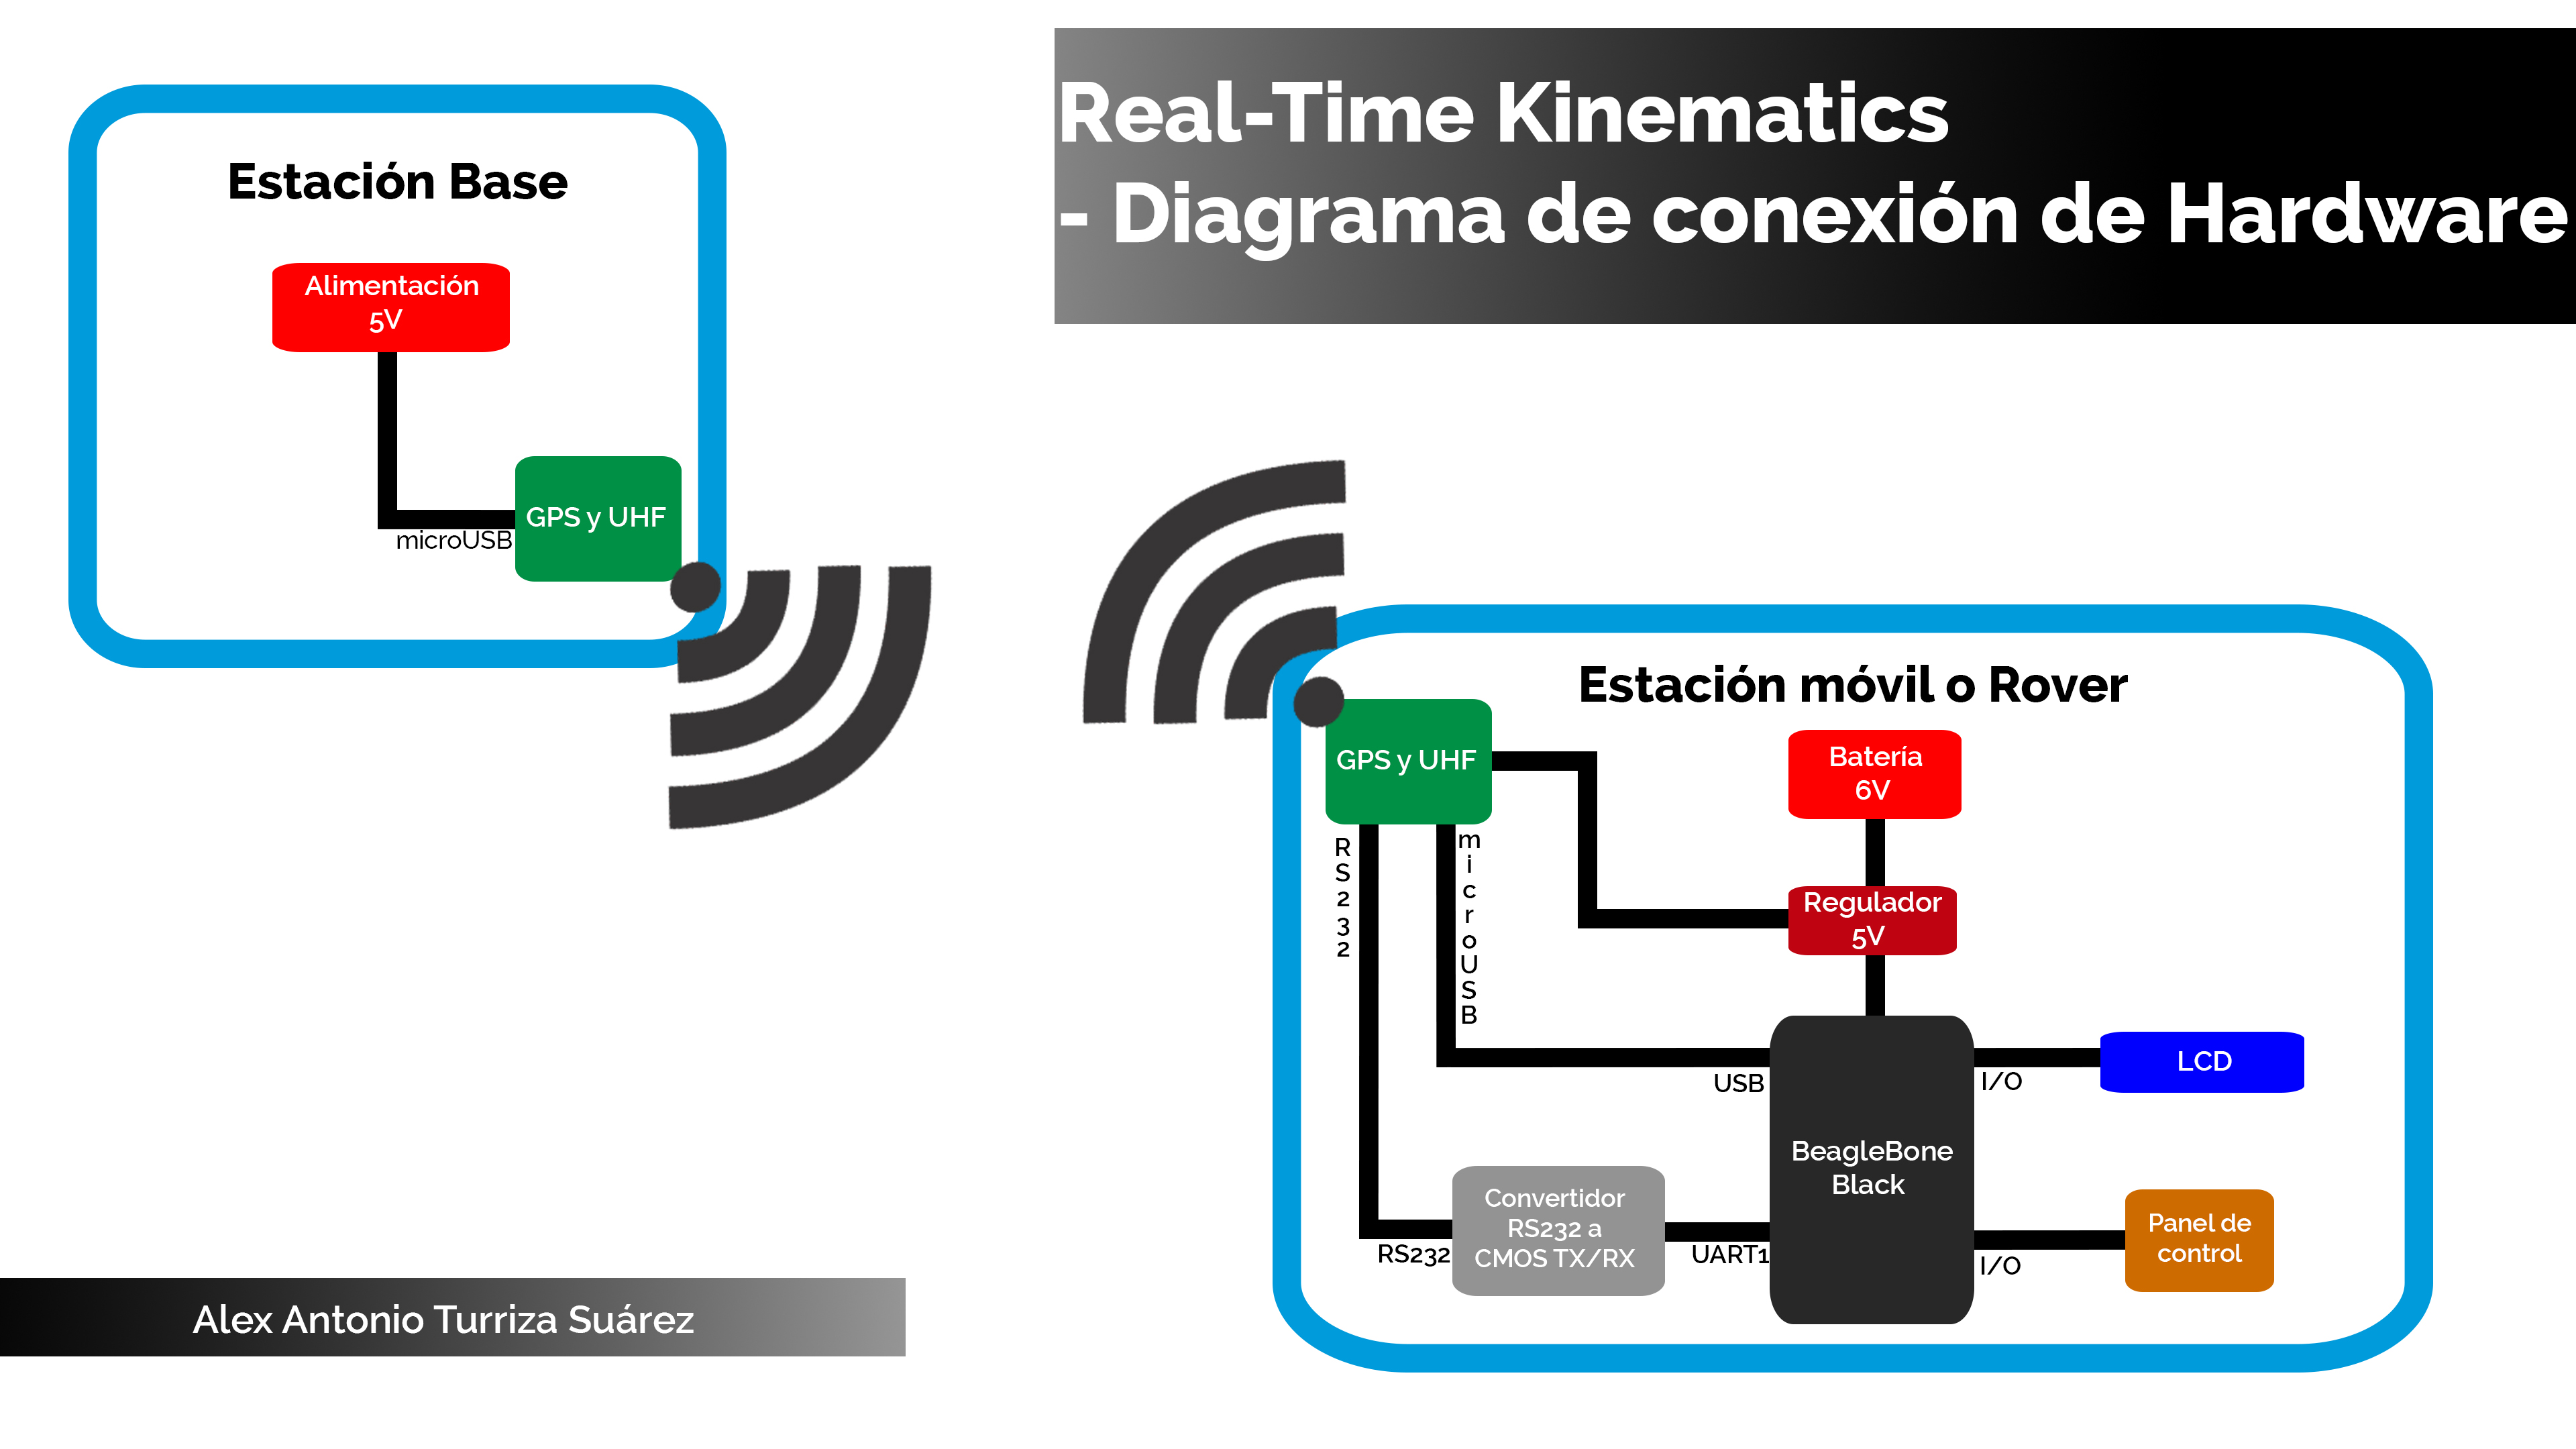
\includegraphics[width=0.95\textwidth]{Figures/DiagFinal}
\caption[Prototipo.]{Prototipo.}
\label{fig:diaghard}
\end{figure}

El sistema cuenta con dos estaciones, tal y como se puede observar en la figura~\ref{fig:diaghard}:  una que es conocida como \textit{estación base} y es la encargada de ofrecer datos de corrección de las observaciones de GPS, y una estación móvil, cuyo posicionamiento se desea conocer. 

\subsection{Descripción de la estación base}

\begin{figure}[H]
\centering
\includegraphics[width=0.95\textwidth]{Figures/BaseStat1}
\caption[Estación base.]{Estación base.}
\label{fig:estbase}
\end{figure}

La estación base cuenta con dos componentes principales:

\begin{itemize}
\item Tarjeta GPS Ublox C94-M8P.
\item Módulo de Comunicación inalámbrica.
\end{itemize}

En la figura~\ref{fig:estbase} se puede observar la estación base en una prueba realizada en el exterior. En la memoria de la tarjeta Ublox C94-M8P de esta estación se encuentran las coordenadas de su posición actual (se pueden actualizar vía PC utilizando el anexo de configuración de los dispositivos GPS Ublox C94-M8P para su uso en RTKLIB en el apéndice~\ref{Anx:ublox}, adjunto a esta tesis).\\

Mediante la comunicación inalámbrica, los datos de posicionamiento necesarios para aplicar correcciones son enviadas a la tarjeta Ublox de la estación móvil, utilizando el protocolo RTCM3.

\subsection{Descripción de la estación móvil}

\subsubsection{Obtención de datos de GPS}

\begin{figure}[H]
\centering
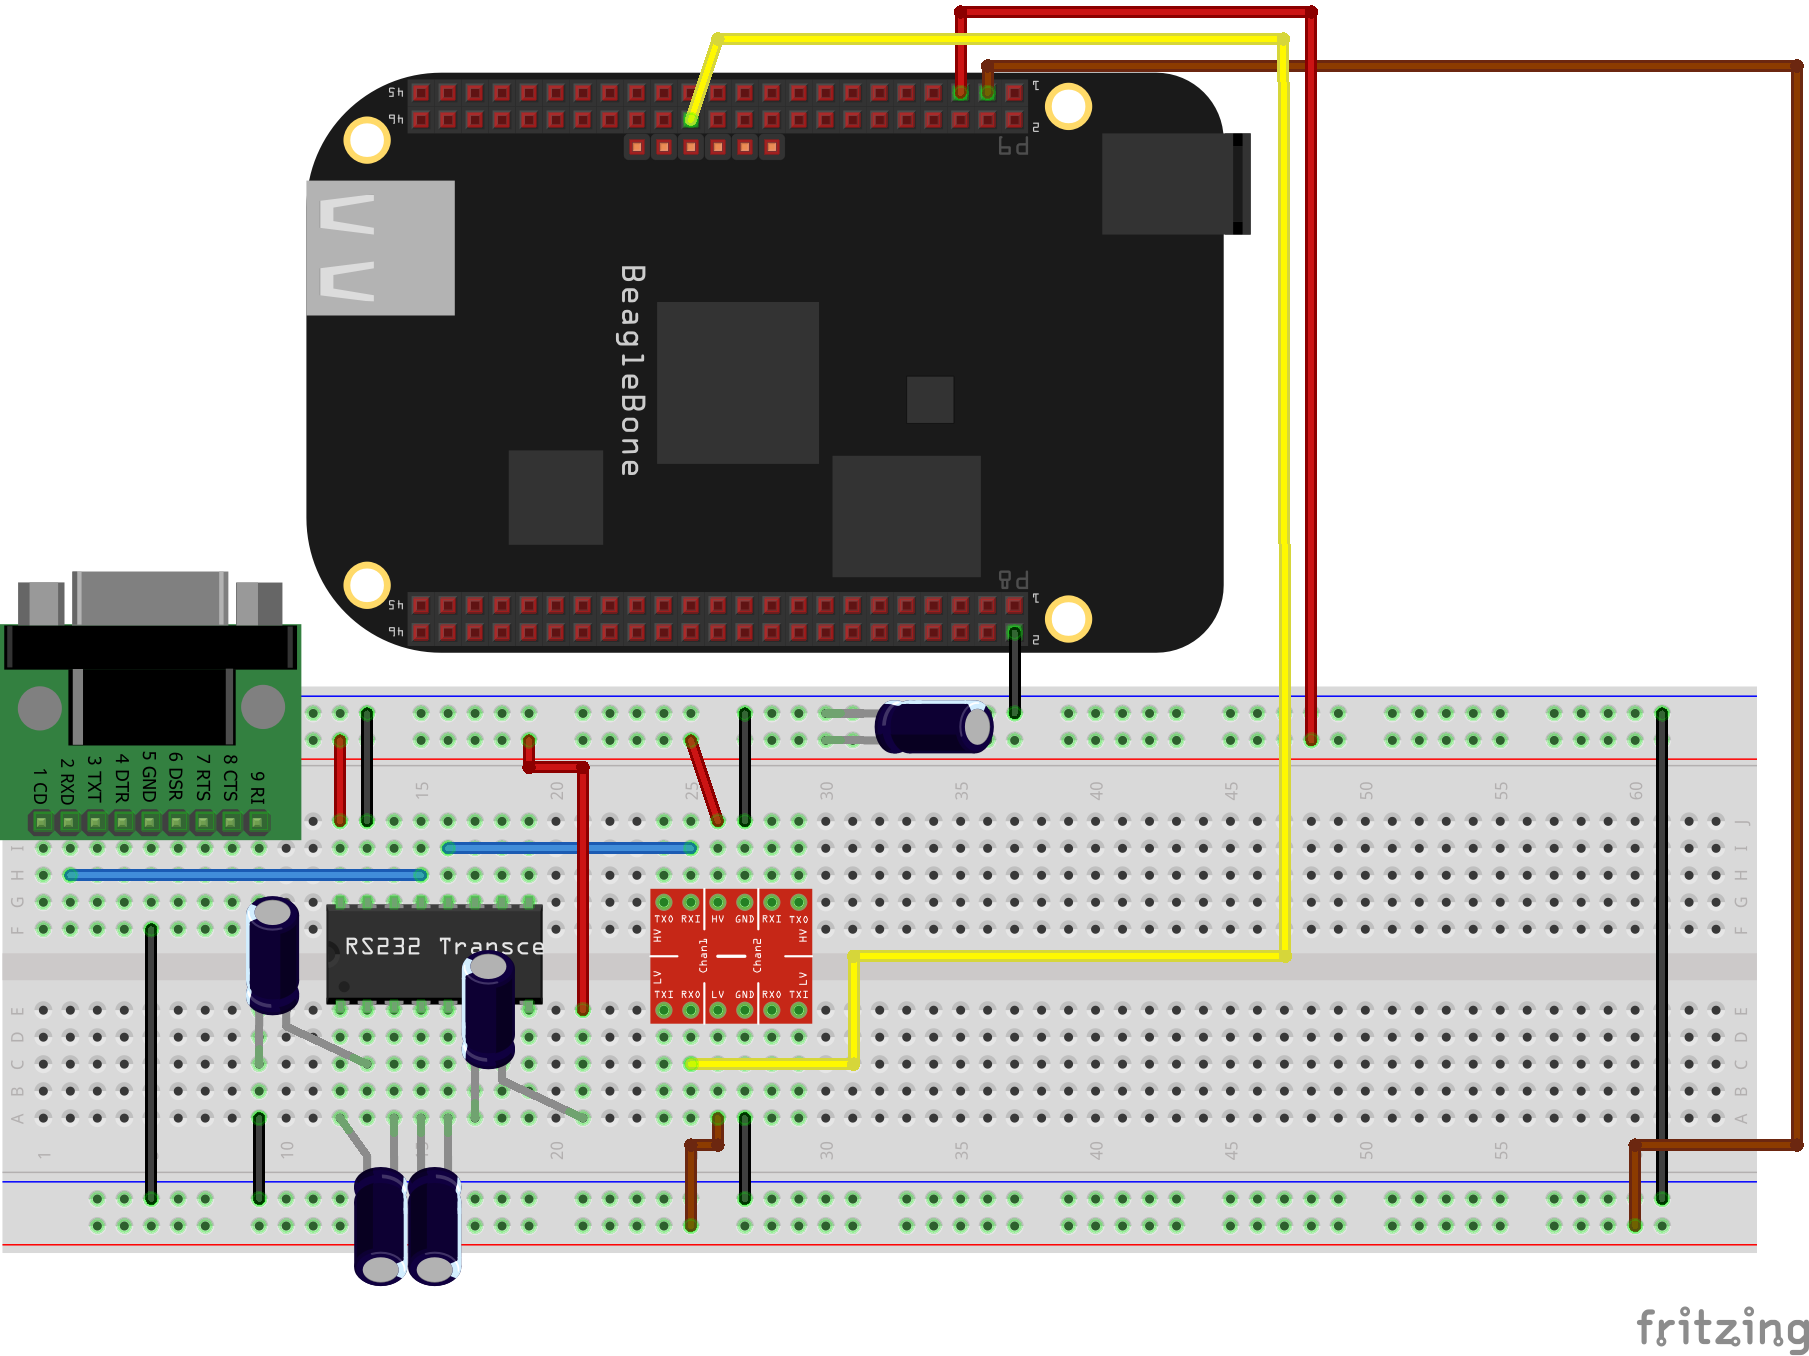
\includegraphics[width=0.95\textwidth]{Figures/Max232}
\caption[Convertidor de RS232 a CMOS RX/TX.]{Convertidor de RS232 a CMOS RX/TX.\footnotemark}
\label{fig:convert}
\end{figure}

\footnotetext{Todos los diagramas de conexión electrónica son para referencia y no muestran el estado real del cableado. Todos fueron realizados con el software fritzing.}

El diseño de los componentes de la estación móvil gira en torno a las capacidades y al diseño del GPS Ublox C94-M8P, de quien se tomarán dos datos importantes: datos de posicionamiento de esta misma tarjeta, ofrecidos por un puerto microUSB, y los datos de corrección de posición proporcionados por la estación base a través de comunicación inalámbrica, obtenidos por protocolo RS232, a través de un periférico como el que se muestra en la figura~\ref{fig:convert}. Por tanto, en la tarjeta BeagleBone Black, son reservados el puerto USB y un puerto (dos pines) de comunicación serial.\\

\subsubsection{Visualización de resultados}

Para la visualización de los datos durante el funcionamiento del sistema, se dispone de una pantalla LCD 16x2 RGB conectada a pines de entrada/salida de uso general de la BeagleBone de la forma que muestra la siguiente figura~\ref{fig:LCDCon}. En la figura~\ref{fig:LCDFunc}, se puede observar dicha LCD proporcionando datos ya procesados de localización:

\begin{figure}[H]
\centering
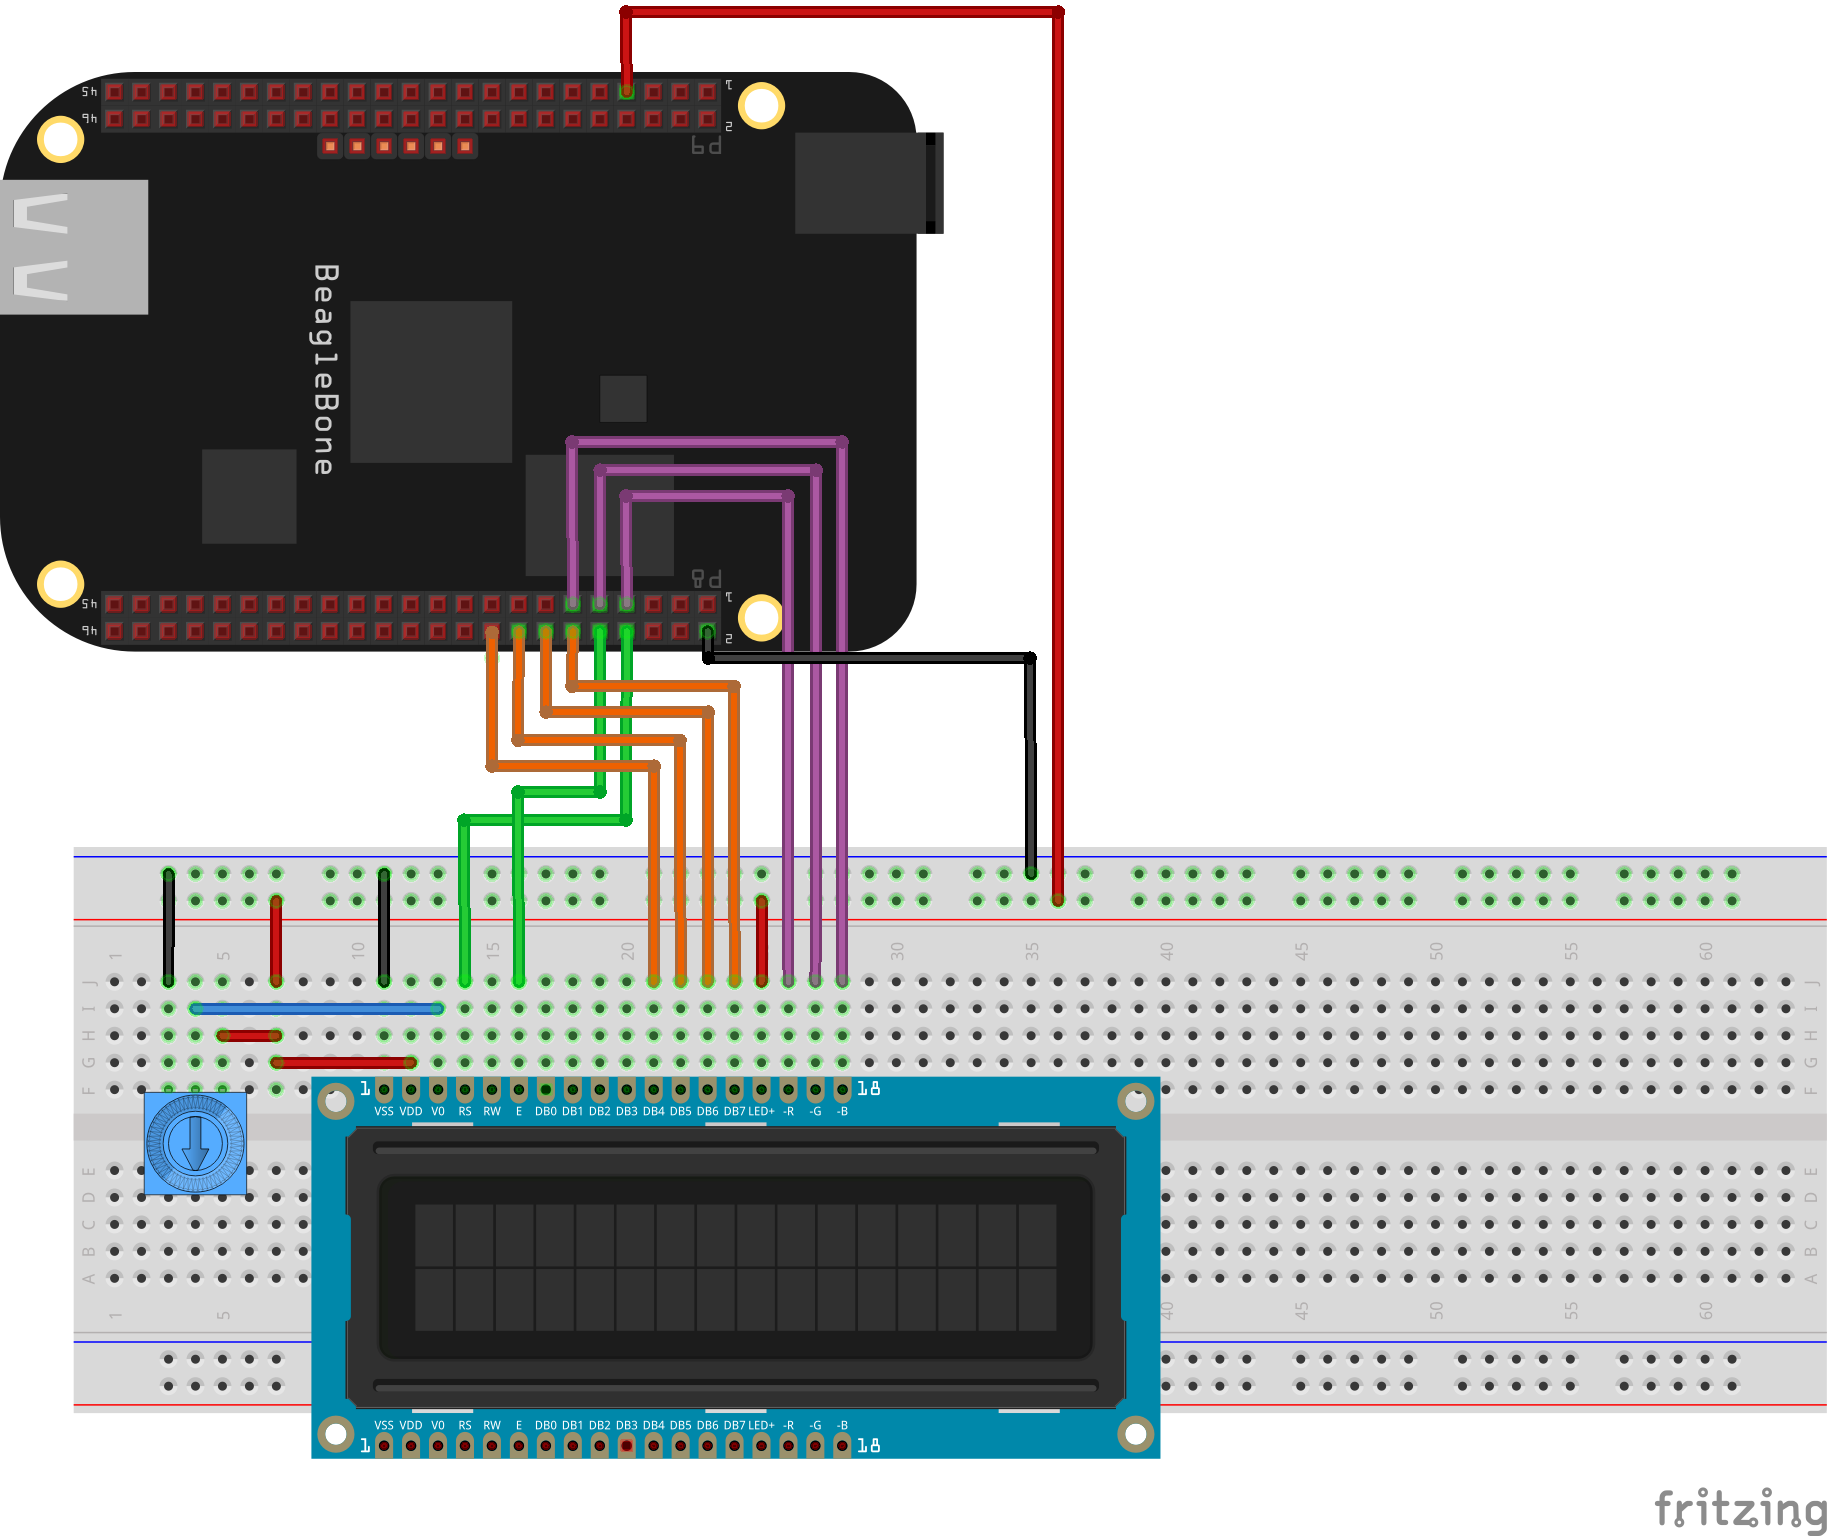
\includegraphics[width=0.95\textwidth]{Figures/LCD_Con}
\caption[Conexión de la LCD.]{Conexión de la LCD.}
\label{fig:LCDCon}
\end{figure} 

\begin{figure}[H]
\centering
\includegraphics[width=0.95\textwidth]{Figures/LCD}
\caption[LCD proporcionando información de posicionamiento.]{LCD proporcionando información de posicionamiento.}
\label{fig:LCDFunc}
\end{figure}

También, para un mejor control de estados del programa, se dispone de dos push buttons y un diodo LED conectados cada uno a pines de entrada/salida de uso general en la BeagleBone, tal y como muestra el circuito de la figura~\ref{fig:ContPan}.

\begin{figure}[H]
\centering
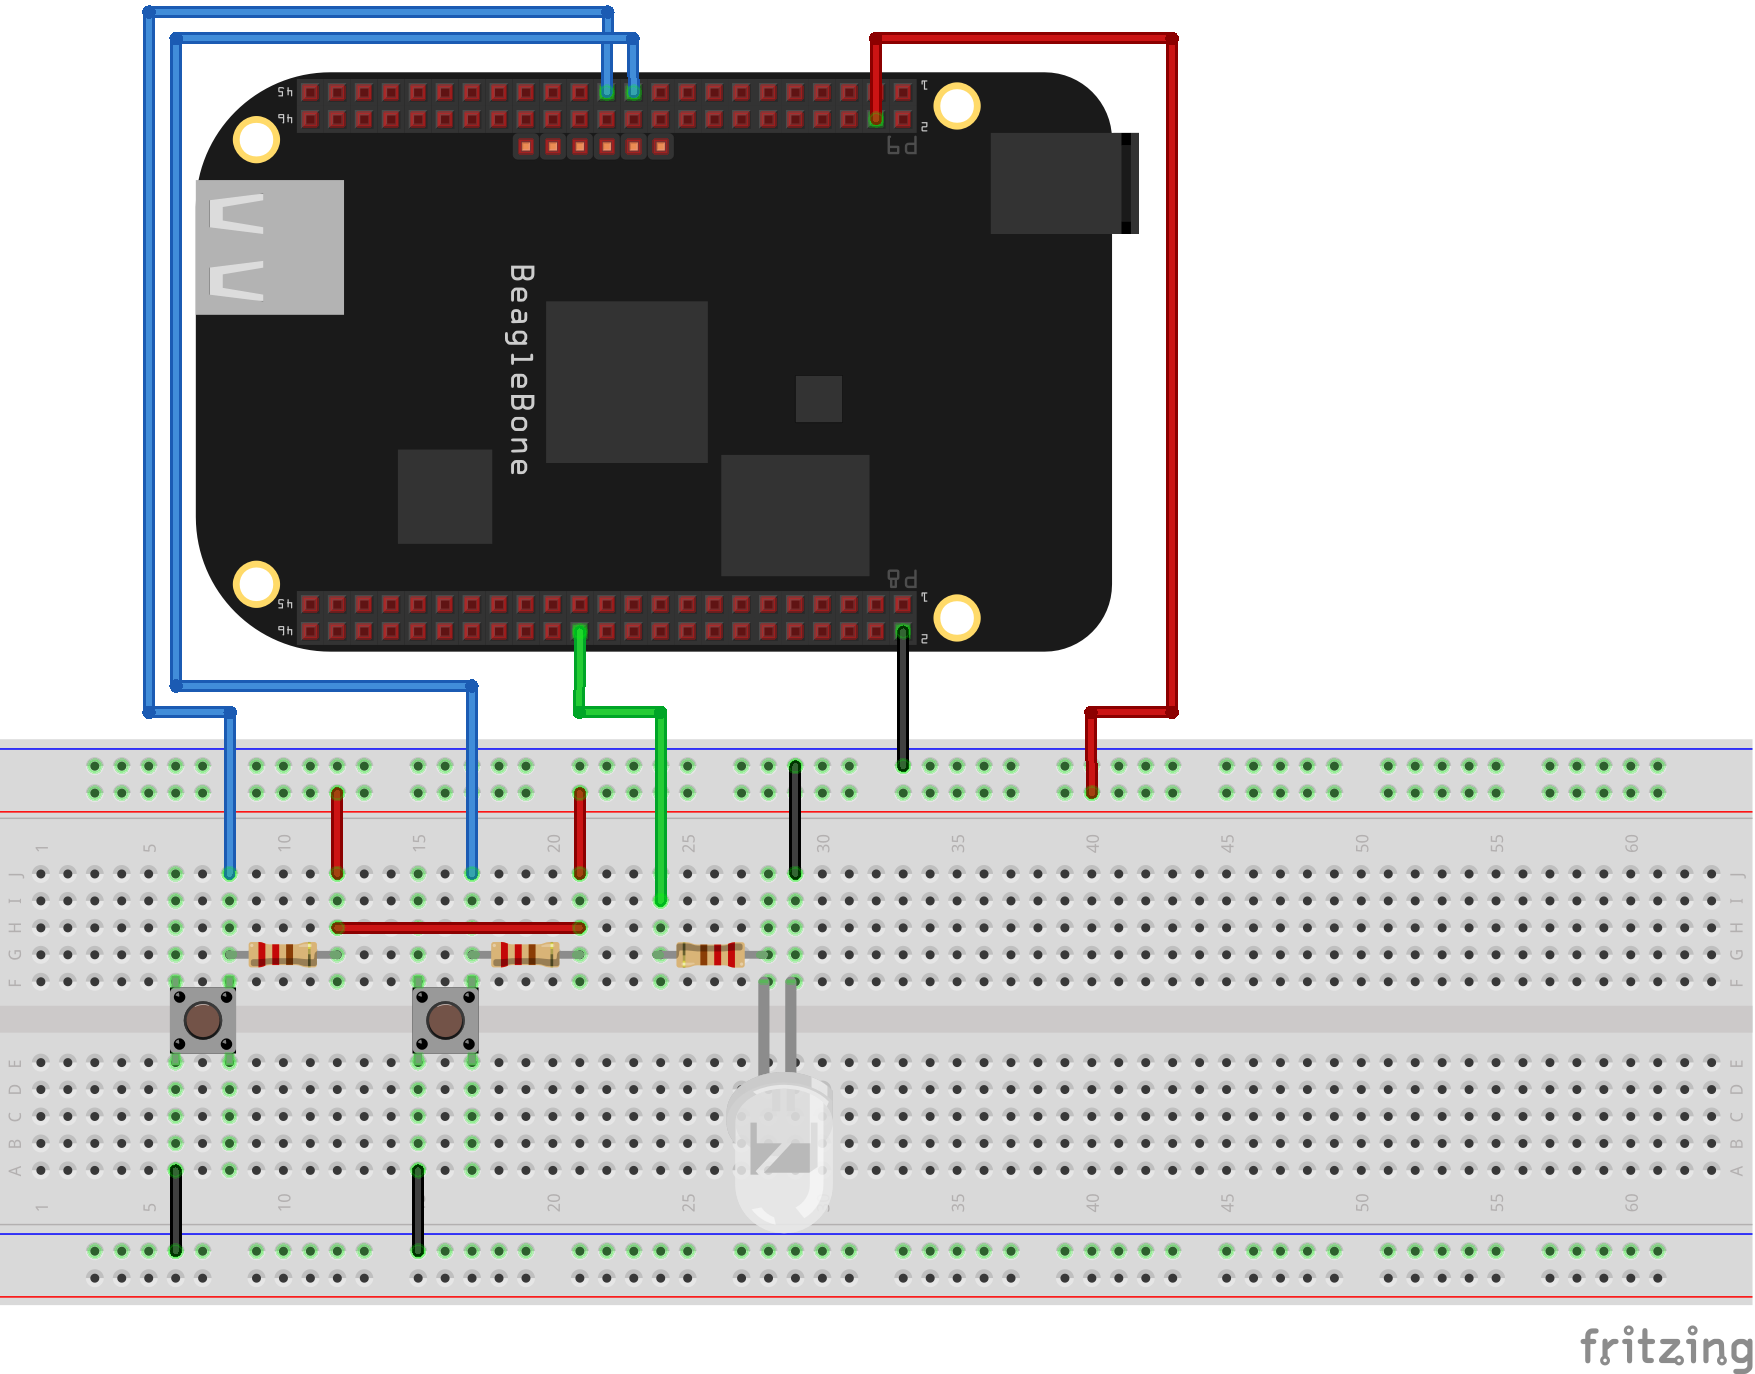
\includegraphics[width=0.95\textwidth]{Figures/ControlPanel}
\caption[Panel del Control.]{Panel de Control.}
\label{fig:ContPan}
\end{figure}

\section{Software}

En el apartado de software, se cuenta con dos conjuntos importantes de código: \textbf{RTKLIB} y bibliotecas para manejo de los pines de entrada/salida de uso general. Mediante estos últimos, fueron implementados los programas que controlan a los diversos periféricos de hardware conectados, incluido el GPS.

\subsection{RTKLIB}

Para una correcta implementación de RTKLIB\footnotemark en la BeagleBone Black, basada en arquitectura ARM, se pasó por distintas etapas:\\

\footnotetext{La versión utilizada es la beta 26 de RTKLIB en su versión 2.4.3, dado que es a partir de estas betas que se da soporte a los mensajes proporcionados por Ublox C94-M8P}

\begin{itemize}
\item \textbf{Configuración en Windows x86\_64:} Dadas las facilidades ofrecidas por RTKLIB en este sistema operativo (dos de ellas y las más importantes, el entorno gráfico y la cantidad de documentación) se decidió configurar el sistema primero bajo Windows, como se puede apreciar en la figura~\ref{fig:RTKWin}. \\

\begin{figure}[H]
\centering
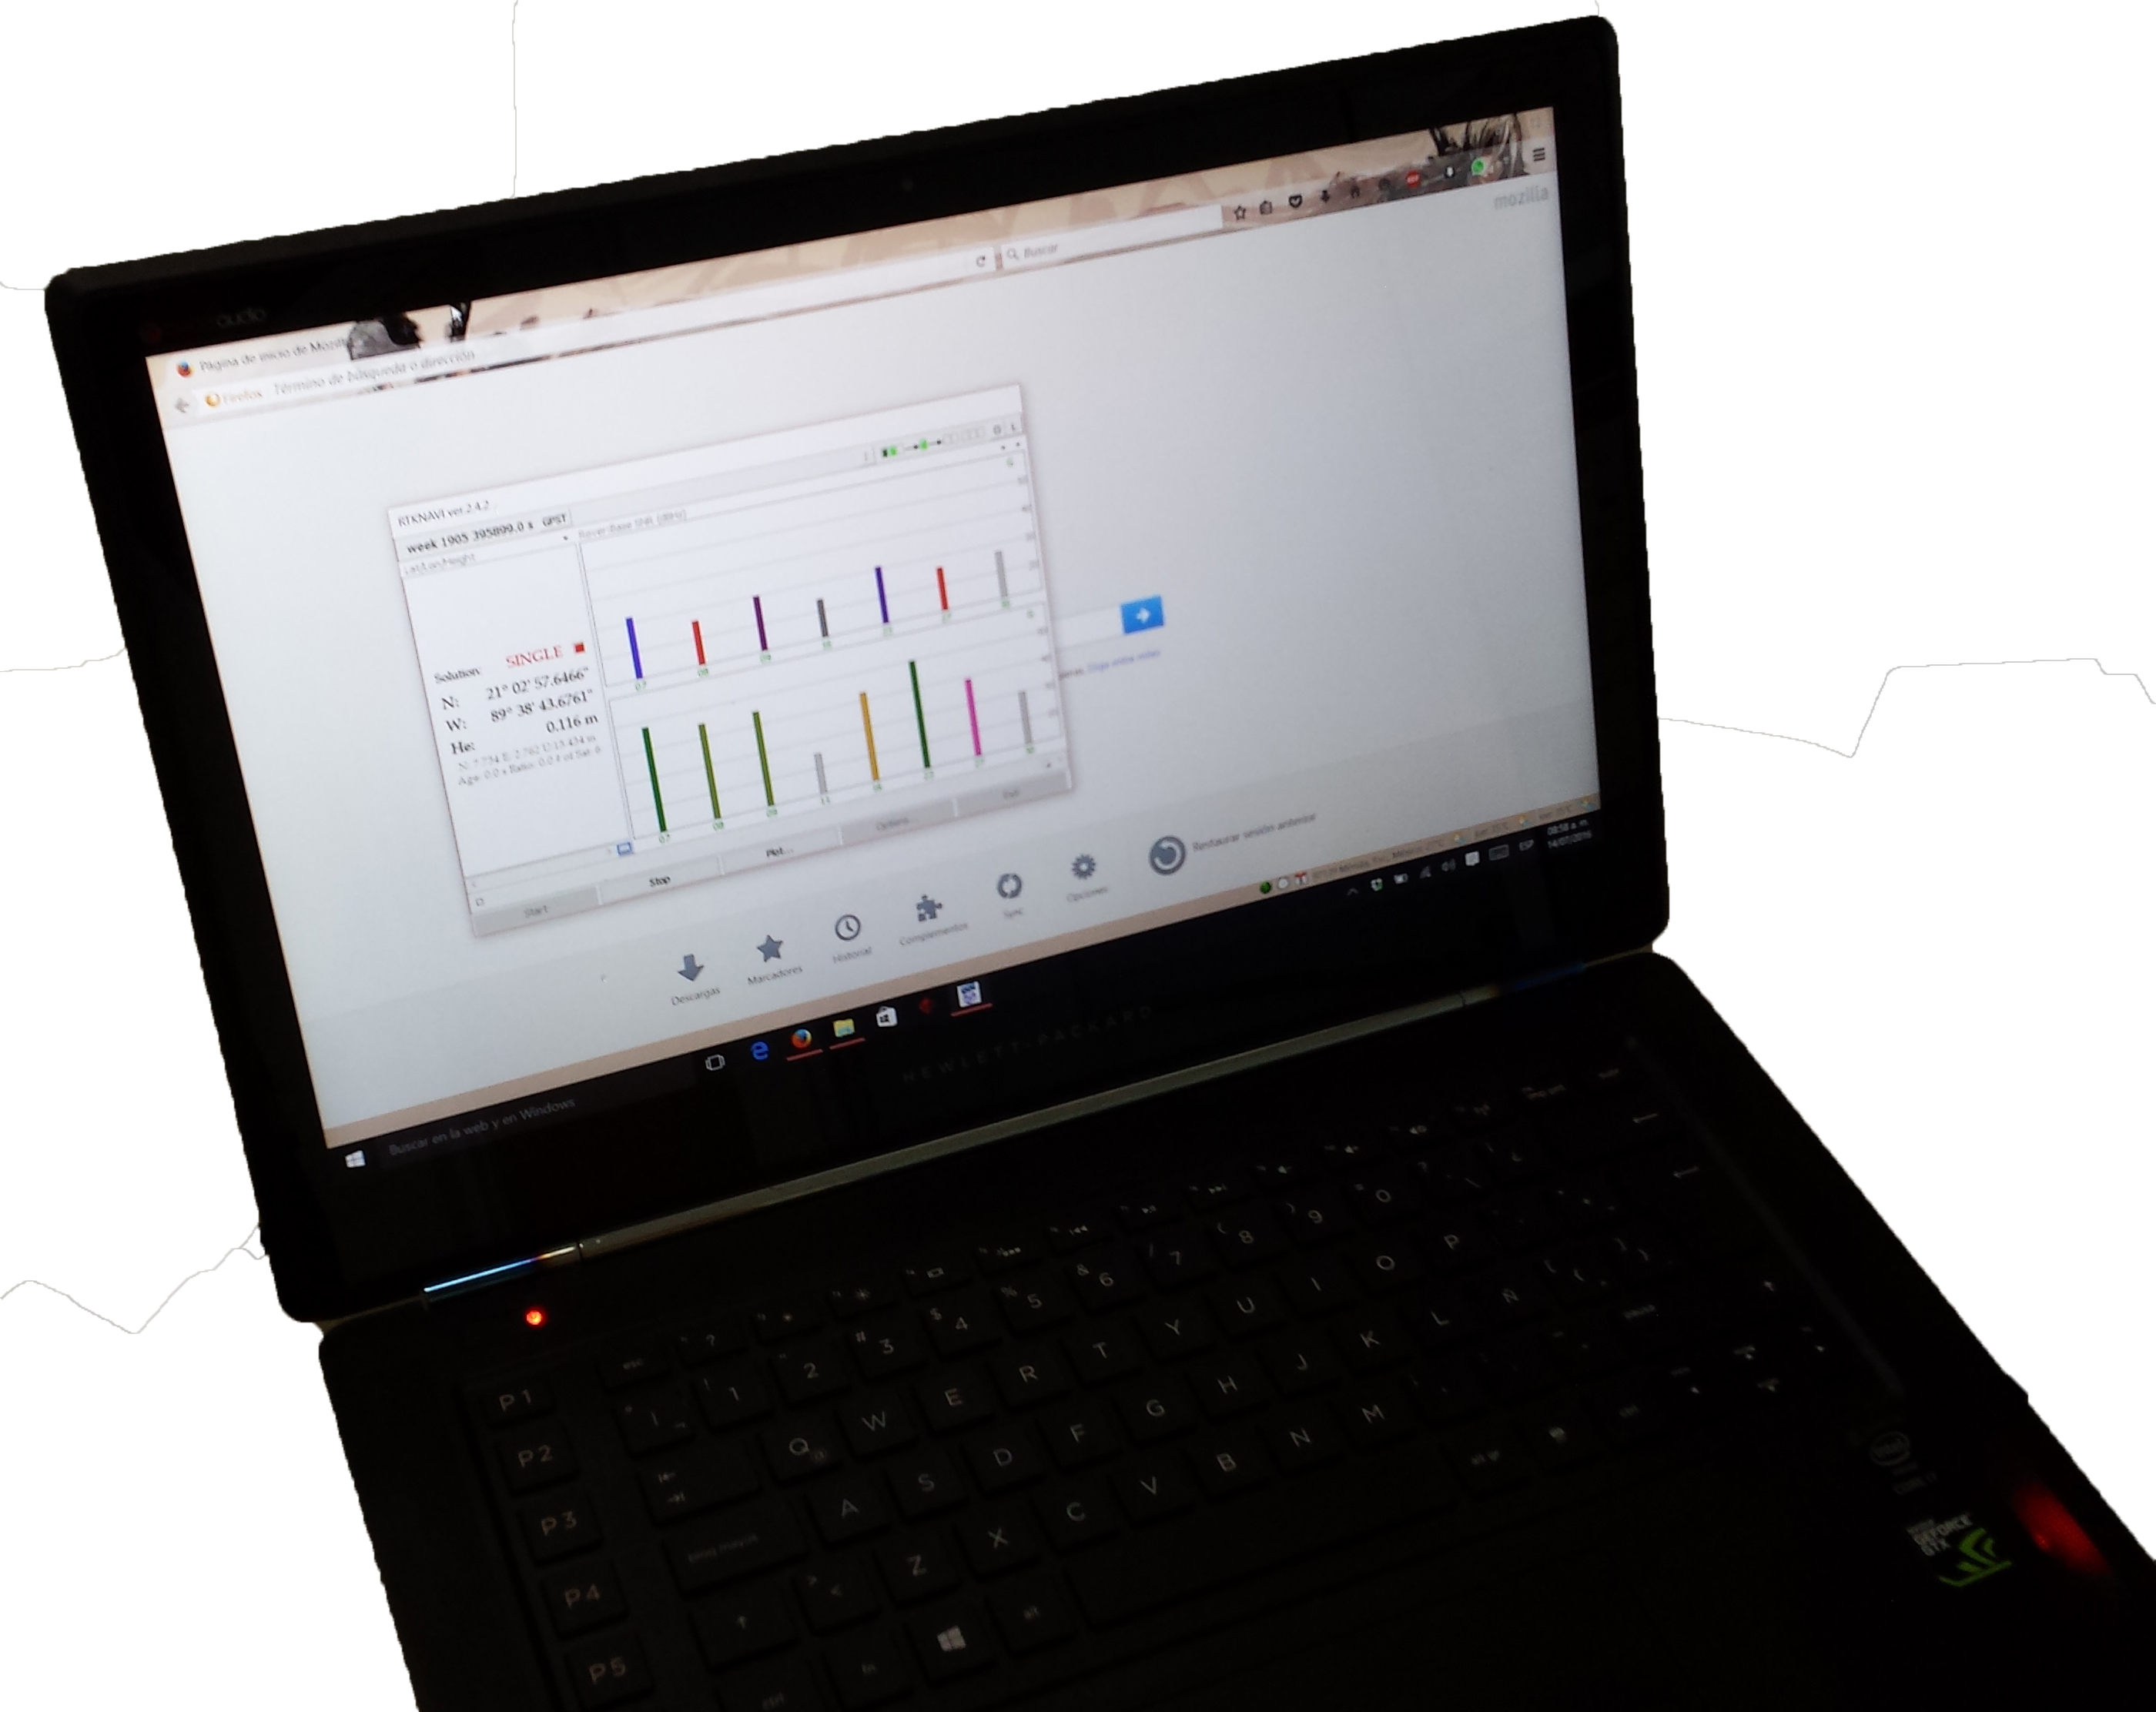
\includegraphics[width=0.95\textwidth]{Figures/BaseStatWin}
\caption[RTKLIB mostrando información de observaciones en Windows.]{RTKLIB mostrando información de observaciones en Windows.}
\label{fig:RTKWin}
\end{figure}

Mediante RTKNAVI, una aplicación de RTKLIB, se configuró el entorno para que reconociese los mensajes de GPS a través de USB, los distintos modos de funcionamiento, y cómo otorgaba los datos ya procesados, además de observación de geolocalización mediante un mapa al momento de la puesta en marcha.\\

\item \textbf{Hacer funcionar el sistema en GNU/Linux x86\_64:} Una vez funcionando RTKLIB en Windows, el objetivo de este punto es el de transportarse a un sistema intermedio entre el utilizado por el dispositivo de destino y el de donde se configuró inicialmente, sabiendo que todo el hardware estaba correctamente conectado y funcionando.\\ 

Bajo este Sistema Operativo, la aplicación RTKRCV, que es la equivalente en entorno consola a RTKNAVI en Windows, es la encargada de procesar los datos de la tarjeta GPS Ublox C94-M8P. Se realizaron los ajustes necesarios para hacer operativo el hardware, tales como indicar las rutas de obtención de datos.\\

Una captura de pantalla de RTKRCV funcionando puede verse en la figura~\ref{fig:rtkrcv1}.

\begin{figure}[H]
\centering
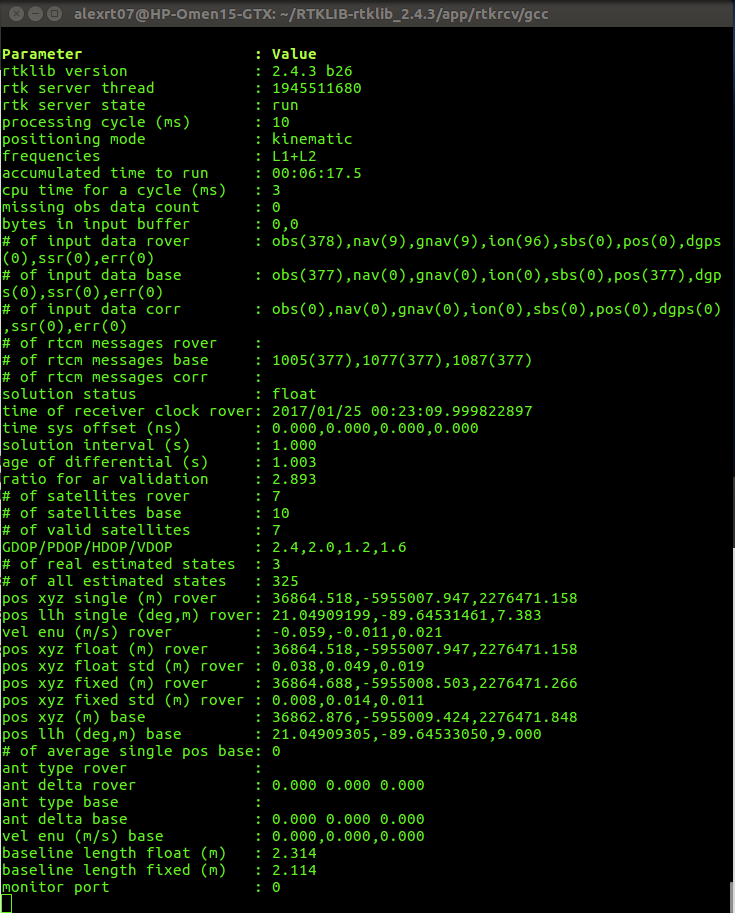
\includegraphics[width=0.85\textwidth]{Figures/LLH}
\caption[RTKRCV funcionando en GNU\_Linux PC.]{RTKRCV funcionando en GNU\_Linux PC.}
\label{fig:rtkrcv1}
\end{figure}

\item \textbf{Hacer funcionar el sistema en GNU/Linux ARM:} Una vez configurado correctamente para GNU/Linux en el punto anterior, sólo quedaba conectar todo a la microcomputadora BeagleBone y verificar que todo funcionase como en la PC. Los datos de salida de RTKLIB son ofrecidos vía socket y son recibidos a través de otro programa codificado en C++.
\end{itemize}

\subsection{Biblioteca BlackGPIO}

La biblioteca BlackGPIO fue desarrollada por Yigit Yuce\footnotemark para poder tener un control ordenado de los puertos de la BeagleBone a través de programación en C++. Utilizándole, se crearon otras dos bibliotecas a partir de las cuales se pueden instanciar objetos conectados a la microcomputadora.

\footnotetext{\href{https://github.com/yigityuce/BlackLib}{https://github.com/yigityuce/BlackLib}}

\subsubsection{Biblioteca GPS}

La biblioteca GPS \textit{gps.h} es utilizada para instanciar un objeto de tipo GPS que contiene en sus atributos distintos strings que contendrán datos de observaciones tales como longitud y latitud. Incluye también un buffer de lectura que utiliza internamente para la asignación de los anteriores valores.\\

Entre sus métodos están conjuntos de sets y gets para manejo de información. Todos están protegidos con exclusiones mutuas que evitan que información errónea sea entregada.

\subsubsection{Biblioteca LCD}

La biblioteca LCD \textit{lcd.h} permite instanciar una LCD RGB de 16x2 conectada a los pines que se le indiquen al constructor siguiendo el orden de declaración que se indica: rojo, verde, azul, RS, enable, db7, db6, db5, db4. Durante el proceso de instanciación del objeto, automáticamente se inicializa para el inmediato despliegue de información en  la siguiente línea de código.Entre sus métodos se encuentra el apagar y encender la pantalla, cambiar el color, escribir un string en la pantalla, saltos de línea, etcétera.

\section{Conclusión}

Una vez detallado cómo funciona el sistema y el papel que juega cada componente, se procede a definir el ejercicio al cual es sometido el sistema para la obtención de resultados.\\
 
En el capítulo~\ref{Chap:DisExp} se hablará acerca de los experimentos realizados y el cómo fueron diseñados, además de los resultados esperados.